%!TEX root = IntroArithGrps.tex






\mychapter{Ratner's Theorems\texorpdfstring{\\}{ }on Unipotent Flows}
\label{RatnerChap}

\prereqs{none.}


This chapter presents three theorems that strengthen and vastly generalize the  well-known and useful observation that if $V$ is any straight line in the Euclidean plane~$\real^2$, then the closure of the image of~$L$ in~$\torus^2$ is a very nice submanifold \csee{LineDenseInT2}. The plane can be replaced with any Lie group~$H$, and $V$ can be any subgroup of~$H$ that is generated by unipotent elements.


\section{Statement of Ratner's Orbit-Closure Theorem}

\begin{eg} \label{LineDenseInT2}
 Let 
 	\begin{itemize}
	\item $V$ be any $1$-dimensional subspace of the vector space~$\real^2$,
	\item $\torus^2   = \real^2 / \integer^2$ be the ordinary $2$-torus,
	\item $x \in \torus^2$,
	and
	\item $\pi \colon \real^2 \to \torus^2$ be the natural covering map.
	\end{itemize}
Geometrically, $V + x$~is a straight line in the plane, and it is classical (and not difficult to prove) that:
	\begin{enumerate}
	\item \label{LineDenseInT2-notdense}
If the slope of the line $V + x$ is rational, then $\pi(V + x)$ is closed, and it is homeomorphic to the circle~$\torus^1$ \csee{LineDenseInT2-notdenseExer}. 
	\item \label{LineDenseInT2-dense}
If the slope of the line $V + x$ is irrational, then the closure of $\pi(V + x)$ is the entire torus~$\torus^2$ \csee{LineDenseInT2-denseExer}. 
	\end{enumerate}
\end{eg}

An analogous result holds in higher dimensions: 
if we take any vector subspace of~$\real^\ell$, the closure of its image in~$\torus^\ell$ will always be a nice submanifold of~$\torus^\ell$. Indeed, the closure will be a subtorus of~$\torus^\ell$: 

\begin{eg}[\csee{SubspaceInTellExer}] \label{SubspaceInTell}
Let 
	\begin{itemize}
	\item $V$ be a vector subspace of~$\real^\ell$,
	\item $\torus^\ell   = \real^\ell / \integer^\ell$ be the ordinary $\ell$-torus,
	\item $x \in \torus^\ell$,
	and
	\item $\pi \colon \real^\ell \to \torus^\ell$ be the natural covering map.
	\end{itemize}
Then the closure of $\pi(V + x)$ in~$\torus^\ell$ is homeomorphic to a torus~$\torus^k$ (with $0\le k \le \ell$\,).  

More precisely, there is a vector subspace~$L$ of~$\real^\ell$, such that
	\begin{itemize}
	\item the closure of $\pi(V + x)$ is $\pi(L + x)$,
	and
	\item $L$ is defined over~$\rational$ (or, in other words, $L \cap \integer^\ell$ is a $\integer$-lattice in~$L$), so $\pi(L + x) \iso L/ (L \cap \integer^\ell)$ is a torus.
	\end{itemize}
 \end{eg}

The above observation about tori generalizes in a natural way to much more general homogeneous spaces, by replacing:
	\begin{itemize}
	\item $\real^3$ with any connected Lie group~$H$,
	\item $\integer^3$ with a lattice~$\Lambda$ in~$H$,
	\item the vector subspace~$V$ of~$\real^3$ with any subgroup of~$H$ that is generated by unipotent elements,
	\item $x + V$ with the coset $x V$,
	\item the map $\pi \colon \real^\ell \to \torus^\ell$ with the natural covering map $\pi \colon H \to H/\Lambda$,
	and
	\item the vector subspace~$L$ of~$\real^\ell$ with a closed subgroup~$L$ of~$H$.
	\end{itemize}
Because it suffices for our purposes, we state only the case where $H$ is semisimple (so we call the group~$G$, instead of~$H$):

\begin{namedthm}[Ratner's Orbit-Closure Theorem] \label{Ratner-OrbitClosure}
	\thmindex{Ratner's!Orbit-Closure}
Suppose
	\begin{itemize}
	\item $V$ is a subgroup of~$G$ that is generated by unipotent elements, 
	and
	\item $x \in G/\Gamma$.
	\end{itemize}
Then there is a closed subgroup~$L$ of~$G$, such that  the closure of\/ $V x$ is~$L x$. 

Furthermore, $L$~can be chosen so that:
	\begin{enumerate}
	\item $L$ contains the identity component of\/~$V$,
	\item \label{Ratner-OrbitClosure-AlmConn}
	$L$ has only finitely many connected components,
	and
	\item \label{Ratner-OrbitClosure-probmeas}
there is an $L$-invariant, finite measure on $L x$.
	\end{enumerate}
\end{namedthm}

(Also note that $L x$ is closed in $G/\Gamma$, since it is the closure of~$Vx$.)


\begin{rem} 
Write $x = g \Gamma$, for some $g \in G$, and let $\Lambda = (g\Gamma g^{-1}) \cap L$.
	\begin{enumerate}
	\item The theorem tells us that the closure of $V x$ is a very nice submanifold of $G/\Gamma$. Indeed, the closure is homeomorphic to the homogeneous space $L/\Lambda$\,.
	\item Conclusion~\pref{Ratner-OrbitClosure-probmeas} of the theorem is equivalent to the assertion that $\Lambda$ is a lattice in~$L$.
	\end{enumerate}
\end{rem}

\begin{warn} \label{MustBeUnip}
The assumption that $V$ is generated by unipotent elements cannot be eliminated. For example, it is known that if $V$ is the group of diagonal matrices in $G = \SL(2,\real)$, then there are points $x \in G/\SL(2,\integer)$, such that the closure of $V x$ is a \term{fractal}. This means that the closure of $V x$ can be a very bad set that is not anywhere close to being a submanifold.
\end{warn}

Unfortunately, the known proofs of Ratner's Orbit-Closure Theorem are rather long. 
One of the paramount ideas in the proof will be described in \cref{RatnerShearingSect}, but, first, we will present a few of the theorem's applications (in \cref{RatnerApplsSect}) and state two other variants of the theorem (in \cref{RatnerVariantsSect}).

\begin{exercises}

\item \label{LineDenseInT2-notdenseExer}
Verify \fullcref{LineDenseInT2}{notdense}.

\item \label{LineDenseInT2-denseExer}
Verify \fullcref{LineDenseInT2}{dense}.

\item \label{SubspaceInTellExer}
Verify \cref{SubspaceInTell}.

\item Show that if $V$ is connected, then the subgroup~$L$ in the conclusion of \cref{Ratner-OrbitClosure} can also be taken to be connected.

\item \label{NonDivergeEx}
(Non-divergence of unipotent flows)
Suppose 
	\begin{itemize}
	\item $\{u^t\}$ is a unipotent one-parameter subgroup of~$G$,
	and
	\item $x \in G/\Gamma$.
	\end{itemize}
Use \cref{Ratner-OrbitClosure} to show there is a compact subset~$K$ of~$G$, such that 
	$$ \text{$\{\, t \in \real \mid u^t x \in K \,\}$ is unbounded.} $$
{\smaller (Hence, \cref{MargulisUnipReturns} is logically a corollary of \cref{Ratner-OrbitClosure}. However, in practice, \cref{MargulisUnipReturns} is used in the proof of \cref{Ratner-OrbitClosure}.\par}
\hint{Conclusion~\pref{Ratner-OrbitClosure-probmeas} of \cref{Ratner-OrbitClosure} is crucial.}

\item Show, by providing an explicit counterexample, that the assumption that $\{u^t\}$ is unipotent cannot be eliminated in \cref{NonDivergeEx}.
\hint{Consider the one-parameter group of diagonal matrices in $\SL(2,\real)$, and let $\Gamma = \SL(2,\integer)$.}


\end{exercises}





\section{Applications} \label{RatnerApplsSect}

We will briefly describe just a few of the many diverse applications of Ratner's Orbit-Closure Theorem \pref{Ratner-OrbitClosure}.


\subsection{Closures of totally geodesic subspaces} \ 

\noindent \begin{minipage}{2.6in}
\hbox to 0pt{\hskip 2.65in\vbox to 0pt{
\begin{minipage}{2in}
\vskip 0.1in
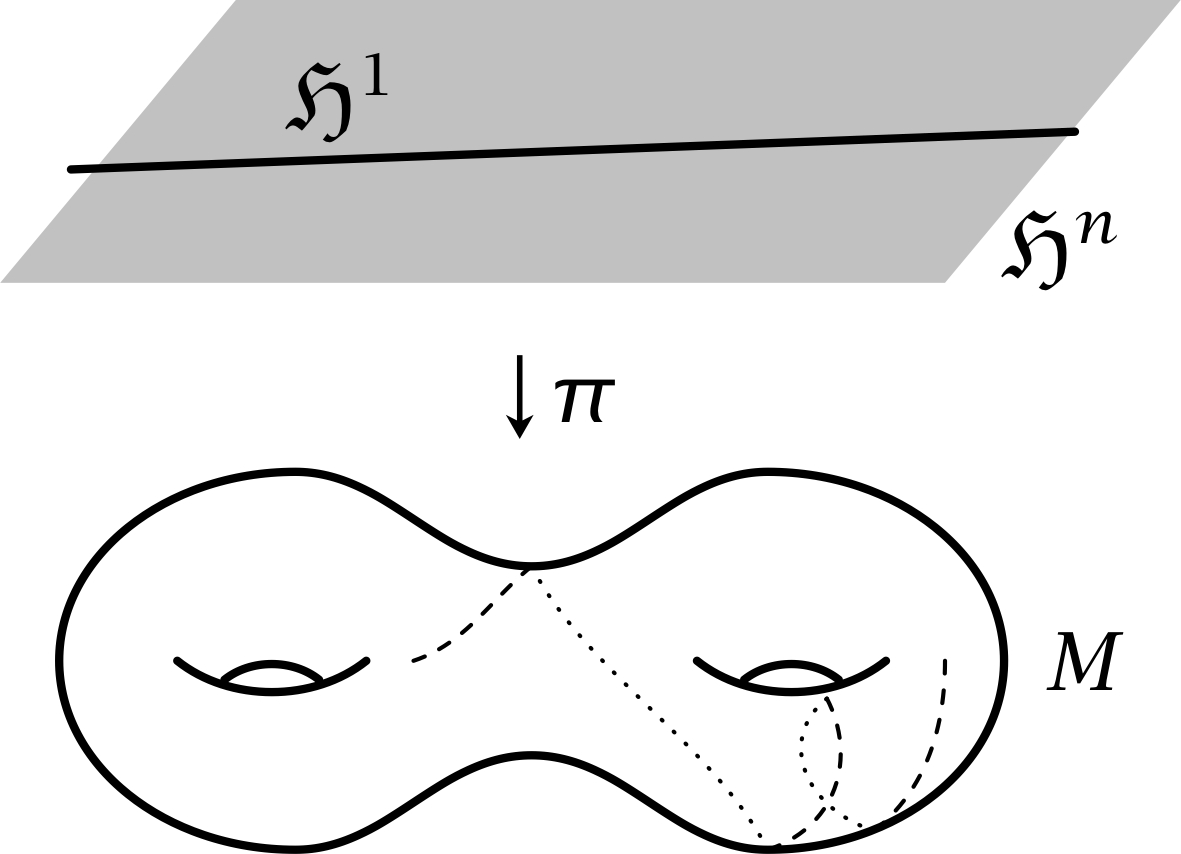
\includegraphics{PDF/H3cover.jpg}\hss
%\\ A line in $\hyperbolic^n$ maps to a curve in a compact, hyperbolic $n$-manifold.
%texpreamble
%("\usepackage[LY1]{fontenc}
% \usepackage[expert, LY1, mylucidascale]{mylucidabr} % I adjusted the scaling
% \usepackage{amsmath}
% \everymath{\displaystyle}
% \usepackage{amssymb}
%\DeclareFontFamily{U}{euF}{}
%\DeclareFontShape{U}{euF}{m}{n}{%
% <-5>*[1.2]eufm5%
% <5-10>gen*[1.2]eufm%
% <10->*[1.2]eufm10%
% }{}
%\DeclareFontShape{U}{euF}{b}{n}{%
% <-5>*[1.2]eufb5%
% <5-10>gen*[1.2]eufb%
% <10->*[1.2]eufb10%
% }{}
% \DeclareMathAlphabet{\AMSfrak}{U}{euF}{m}{n}
% \SetMathAlphabet{\AMSfrak}{bold}{U}{euF}{b}{n}
% ");
%
%from graph access *;
%
%defaultpen(  fontcommand("\normalfont") + fontsize(10) ); 
%
%unitsize(1cm, 0.8cm);
%
%currentpen=linewidth(1);
%
%pair A = (0,0), B = (1,-1), C = (2,-0.5), D = (3,-1), E = (4,0), F = (3,1), G = (2,0.5), H = (1,1);
%real s = 1;
%
%
%// genus 2 surface
%
%draw(  A{S}.. tension s .. {E}B{E}.. tension s .. {E}C{E}.. tension s .. {E}D{E}.. tension s .. {N}E{N}.. tension s .. {W}F{W}.. tension s .. {W}G{W}.. tension s .. {W}H{W}.. tension s .. {S}cycle );
%
%draw( (0.5,-0){SE}..{NE}(1.3,-0) );
%draw( (0.7,-0.1){NE}..{SE}(1.1,-0.1) );
%
%draw( (2.7, 0){SE}..{NE}(3.5, 0) );
%draw( (2.9,-0.1){NE}..{SE}(3.3,-0.1) );
%
%// curve on the surface
%dashed = linetype("3 4");
%draw( (1.5, 0){ENE}..{NE}(2,0.5) , dashed );
%draw( (2,0.5){SSE}..{SSE}(3,-1) , dotted );
%draw( (3,-1){ENE}..{NNW}(3.25,-0.2) , dashed );
%draw( (3.25,-0.2){SW}..{ESE}(3.45,-0.9) , dotted );
%draw( (3.45,-0.9){NE}..{N}(3.75,0) , dashed );
%
%// plane above it
%real x = -0.25, z = 2, l = 4, w = 1.5, d = 1;
%fill( (x, z) -- (x + l,z) -- (x + l + d, z + w) -- (x + d, z + w) -- cycle, gray(0.8) ) ;
%draw( (x + 0.3, z + 0.6) -- ( x + l + 0.55, z + 0.8 ), linewidth(1) );
%
%// downarrow between them, and labels on everything
%
%label( "{\large$\downarrow$}\raise2pt\hbox{$\pi$}", (2.1, 1.4) );
%label( "$M$", (4.35,0) );
%label( "$\AMSfrak{H}^n$", (4.25,2.2) );
%label( "$\AMSfrak{H}^1$", (1.2, 3) );
\end{minipage}
 \vss}\hss}
 \raggedright
\begin{eg} \label{FractalInHyper3Mfld}
 Let $M$ be a  compact, hyperbolic $n$-manifold (with $n \ge 2$).
 \begin{itemize} \itemindent=0pt \leftskip=\parindent
\item There is a covering map $\pi \colon \hyperbolic^n \to M$ that is a local isometry.
\item There is a natural embedding $\iota \colon \hyperbolic^1 \hookrightarrow
\hyperbolic^n$.
\item Let $f_1$ be the composition $\pi \circ \iota$,
 \newline so $f_1 \colon \hyperbolic^1  \to M$.
 \end{itemize}
 \end{eg}
 \end{minipage}

\smallskip

\noindent Then the image of~$f_1$ is a curve in~$M$. It is well known (though not at all obvious) that the closure of this curve can be a very bad set; in fact, even though $\hyperbolic^1$ and~$M$ are nice, smooth manifolds, this closure can be a \term{fractal}. (This is a higher-dimensional analogue of the example in \cref{MustBeUnip}. In the literature, it is the fact that the closure of a geodesic in a compact manifold of negative curvature can be a \term{fractal}.)

It is a consequence of Ratner's Theorem that this pathology never occurs if we replace $\hyperbolic^1$ with a higher-dimensional hyperbolic space:

\begin{cor} \label{GoodClosure(hyper)}
 Let:
 \begin{itemize}
 \item $m,n \in \natural$, with $m \le n$,
 \item $M$ be a  compact, hyperbolic $n$-manifold,
\item $\pi \colon \hyperbolic^n \to M$ be a covering map that is a local isometry,
\item $\iota \colon \hyperbolic^m \hookrightarrow
\hyperbolic^n$ be a totally geodesic embedding,
and
\item $f_m = \pi \circ \iota$, so $f_m \colon \hyperbolic^m  \to M$.
 \end{itemize}
If $m \ge 2$, then the closure $\closure{f_m(\hyperbolic^m)}$ of the image of~$f_m$ is a \textup(totally geodesic\textup) immersed submanifold of~$M$.
\end{cor}

\begin{proof}
We prove only that the closure is a submanifold, not that it is totally geodesic.
Let 
	$$ \text{$V = \SO(1,m)$, \  $G =  \SO(1,n)$, 
	\ and \  $x \in \iota(\hyperbolic^m)$} ,$$
so 
	\begin{itemize}
	\item$G$ acts by isometries on~$\hyperbolic^n$,
	\item $M = \Gamma \backslash \hyperbolic^n$, for some lattice~$\Gamma$ in~$G$,
	and
	\item $\iota(\hyperbolic^m) = V x$.
	\end{itemize}
From Ratner's Orbit-Closure Theorem \pref{Ratner-OrbitClosure}, we know there is a subgroup~$L$ of~$G$, such that 
	$ \closure{\Gamma V} = \Gamma L $.
So 
	$$ \closure{f_m(\hyperbolic^m)}  = \closure{ \pi \bigl( \iota( \hyperbolic^m ) \bigr)}= \closure{\pi(V x)} = \pi(Lx) $$
is an immersed submanifold of~$M$.
\end{proof}

\begin{rems} \label{GoodClosure(LocSymm)} \ 
\begin{enumerate}
\item \label{GoodClosure(LocSymm)-closure}
The same conclusion holds (with the same proof) when $\hyperbolic^m$ and $\hyperbolic^n$ are replaced with much more general symmetric spaces $\cover{X}$ and~$\cover{Y}$ that have no compact factors, except that the closure may not be totally geodesic if $\rank\cover{X} < \rank\cover{Y}$.
\item When $\rank\cover{X} = \rank\cover{Y}$, one proves that the submanifold is totally geodesic by showing that the subgroup~$L$ in the above proof is invariant under the appropriate Cartan involution of~$G$.
\end{enumerate}
\end{rems}


\subsection{Values of quadratic forms}

Many of the most impressive applications of Ratner's Orbit-Closure Theorem (and the related results that will be described in \cref{RatnerVariantsSect}) are in Number Theory. As an example, we present a famous result on values of quadratic forms. It is now an easy corollary of Ratner's Orbit-Closure Theorem, but, historically, it was proved by Margulis before this major theorem was available (by proving the relevant special case of the general theorem).

Let 
	$$ \text{$Q(\vector{x}) = Q(x_1,x_2,\ldots,x_n)$ be a quadratic form in $n$ variables} $$
(in other words, $Q(\vector{x})$ is a homogeneous polynomial of degree~$2$). 

Classical number theorists were interested in determining the values of~$c$ for which the equation $Q( \vector{x}) = c$ has an integer solution; that is, a solution with $\vector{x} \in \integer^n$. For example:
	\begin{enumerate}
	\item Lagrange's 4-Squares Theorem tells us that if
		$$Q(x_1,x_2,x_3,x_4) = x_1^2 + x_2^2 + x_3^2 + x_4^2 ,$$
	then $Q(\vector{x}) = c$ has a solution iff $c \in \integer^{\ge 0}$.
	\item Fermat's 2-Squares Theorem tells us that if $Q(x_1,x_2) = x_1^2 + x_2^2$, and $p$~is an odd prime, then $Q(\vector{x}) = p$ has a solution iff $p \equiv 1 \pmod{4}$.
	\end{enumerate}
These very classical results consider only forms whose coefficients are integers, but we can also look at forms with \emph{irrational} coefficients, such as
	$$ Q(x_1,x_2,x_3,x_4) = 3 x_1^2 - \sqrt{2} x_2 x_3 + \pi x_4^2 .$$
For a given quadratic form $Q(\vector{x})$, it is clear that
	$$ \begin{matrix}
	\text{the equation $Q(\vector{x}) = c$ does not have an integral solution,} \\
	\text{for most real values of~$c$,} 
	\end{matrix} $$
for the simple reason that there are only countably many possible integer values of the variables $x_1,x_2,\ldots,x_n$, but there are uncountably many possible choices of~$c$. Therefore, instead of trying to solve the equation \emph{exactly}, we must be content with solving the equation \emph{approximately}. That is, we will be satisfied with knowing that we can find a value of $Q(\vector{x})$ that is within~$\epsilon$ of~$c$, for every~$\epsilon$ (and every~$c$). In other words, we would like to know that $Q(\integer^n)$ is \emph{dense} in~$\real$.

\begin{egs}
There are some simple reasons that $Q(\integer^n)$ may fail to be dense in~$\real$:
	\begin{enumerate}
	\item Suppose all of the coefficients of $Q(\vector{x})$ are integers. Then we have $Q(\integer^n) \subseteq \integer$, so $Q(\integer^n)$ is obviously not dense in~$\real$. More generally, if $Q(\vector{x})$ is a scalar multiple of a form with integer coefficients, then $Q(\integer^n)$ is not dense in~$\real$.
	\item Suppose all values of $Q(\vector{x})$ are $\ge 0$ (or all are $\le 0$). (In this case, we say that $Q(\vector{x})$ is \defit[positive!definite]{positive-definite} (or \defit{negative-definite}, respectively). For example, this is the case if 
		$$Q(\vector{x}) = a_1 x_1^2 + a_2 x_2^2 + a_3 x_3^2 + \cdots + a_n x_n^2 ,$$
with all coefficients~$a_i$ of the same sign. Then it is clear that $Q(\integer^n)$ is not dense in all of~$\real$.
	\item Let $Q(x_1,x_2) = x_1^2 - \alpha x_2^2$, where $\alpha = 3 + 2 \sqrt{2}$. Then, although it is not obvious, one can show that $Q(\integer^2)$ is not dense in~$\real$ \csee{NotDenseEgEx}. Certain other choices of~$\alpha$ also provide examples where $Q(\integer^2)$ is not dense \csee{BadlyApproxNotDenseEx}, so having only $2$~variables in the quadratic form can cause difficulties.
	\item Even if a form has many variables, there may be a linear change of coordinates that turns it into a form with fewer variables. (For example, letting $z = x + \sqrt{2} y$ transforms $x^2 + 2 \sqrt{2} x y + 2 y^2$ into $z^2$.) A form that admits such a change of coordinates is said to be \defit[quadratic form!degenerate]{degenerate}. Therefore, a degenerate form with more than~$2$ variables could merely be a disguised version of a form with $2$~variables whose image is not dense in~$\real$. 
	\end{enumerate}
\end{egs}

The following result shows that any quadratic form avoiding these simple obstructions does have values that are dense in~$\real$.
It is often called the ``\thmindex{Oppenheim Conjecture}Oppenheim Conjecture\zz,'' because it was an open problem under that name for more than 50 years, but that terminology is no longer appropriate, since it is now a theorem.

\begin{cor}[(Margulis' Theorem on Values of Quadratic Forms)] \label{OppenheimConj}
	\thmindex{Margulis!Values of Quadratic Forms}
Let $Q(\vector{x})$ be a quadratic form  in $n \ge
3$~variables, and assume $Q(\vector{x})$ is:
	\begin{itemize}
	\item not a scalar multiple of a form with integer coefficients,
	\item neither positive-definite nor negative-definite,
	and
	\item nondegenerate.
	\end{itemize}
Then  $Q (\integer^n)$  is dense  in~$\real$.
\end{cor}

\begin{proof}
For simplicity, assume $n = 3$. Let
	\begin{itemize}
	\item $G = \SL(3,\real)$,
	and
	\item $H = \SO(Q)^\circ = \{\, h \in G \mid \text{$Q( h \vector{x} ) = Q(\vector{x})$ for all $\vector{x} \in \real^3$} \, \}^\circ$.
	\end{itemize}
Since $Q(\vector{x})$ is nondegenerate, and neither positive-definite nor negative-definite, we have $H \iso \SO(1,2)^\circ \iso \PSL(2,\real)$, so $H$~is generated by unipotent elements. Furthermore, calculations in Lie theory (which we omit) show that the only connected subgroups of~$G$ containing~$H$ are the obvious ones: $H$ and~$G$. Therefore, Ratner's Orbit-Closure Theorem \pref{Ratner-OrbitClosure} tells us that either:
	\begin{itemize}
	\item $H G_{\integer}$ is closed, and $G_{\integer} \cap H$ is a lattice in~$H$,
	or
	\item the closure of $H G_{\integer}$ is all of~$G$.
	\end{itemize}
However, if $H_{\integer} = G_{\integer} \cap H$ is a lattice in~$H$, then the Borel Density Theorem \pref{BDT(Zardense)} implies that $H$~is defined over~$\rational$ \csee{arithlatt->defdQ}.
Then, since $H = \SO(Q)^\circ$, a bit of algebra shows that $Q(\vector{x})$ is a scalar multiple of a form with integer coefficients \csee{DefdQ->ScalarMult}. This is a contradiction.

Therefore, we conclude that  the closure of $H G_{\integer}$ is all of~$G$. In other words,
	$$ \text{$H G_{\integer}$ is dense in~$G$,} $$
so
	$$ \text{$H G_{\integer} (1,0,0)$ is dense in~$G(1,0,0)$.} $$
Since $G_{\integer} (1,0,0)  \subseteq \integer^3$, and $G (1,0,0) = \real^3 \smallsetminus \{0\}$, this tells us that
	$$ \text{$H \integer^3$ is dense in $\real^3$.} $$
Then, since $Q(\vector{x})$ is continuous, we conclude that
	$$ \text{$Q( H \integer^3 )$ is dense in $Q(\real^3)$.} $$
We also know:
	\begin{itemize}
	\item $Q( H \integer^3 ) = Q(\integer^3)$, by the definition of~$H$,
	and
	\item $Q(\real^3) = \real$, because $Q(\vector{x})$ is neither positive-definite nor negative-definite \csee{Indef->Q(R)=R}.
	\end{itemize}
Therefore $Q(\integer^3)$ is dense in~$\real$.
\end{proof}



\subsection{Products of lattices}

\begin{cor}[\csee{ProdLattsDenseEx}] \label{ProdLattsDense}
If\/ $\Gamma_1$ and\/~$\Gamma_2$ are any two lattices in~$G$, and $G$~is simple, then either
	\begin{enumerate}
	\item $\Gamma_1$ and\/ $\Gamma_2$ are commensurable, so the product\/ $\Gamma_1 \, \Gamma_2$ is discrete,
	or
	\item $\Gamma_1 \, \Gamma_2$ is dense in~$G$.
	\end{enumerate}
\end{cor}



\begin{exercises}

\item \label{BadlyApproxDefnEx}
Suppose $\beta$ is a quadratic irrational. (This means that $\alpha$ is irrational, and that $\alpha$ is a root of a quadratic polynomial with integer coefficients.) Show that $\beta $ is \defit{badly approximable}: i.e., there exists $\epsilon > 0$, such that if $p/q$ is any rational number, then
	$$ \left| \frac{p}{q} - \beta \right| > \frac{\epsilon}{q^2} .$$

\item \label{BadlyApproxNotDenseEx}
Let $Q(x_1,x_2) = x_1^2 - \beta ^2 x_2^2$, where $\beta $ is any badly approximable number \ccf{BadlyApproxDefnEx}. Show that $Q(\integer^2)$ is not dense in~$\real$.
\hint{There exists $\delta > 0$, such that $|Q(p,q)| \ge \delta $ for $p,q \in \integer \smallsetminus \{0\}$.}

\item \label{NotDenseEgEx}
Let $Q(x_1,x_2) = x_1^2 - \alpha x_2^2$, where $\alpha = 3 + 2 \sqrt{2}$. Show $Q(\integer^2)$ is not dense in~$\real$.
\hint{Use previous exercises, and note that $3 + 2 \sqrt{2} = \bigl( 1 + \sqrt{2} \bigr)^2$.}

\item \label{DefdQ->ScalarMult}
Suppose $Q(\vector{x})$ is a nondegenerate quadratic form in $n$~variables.
Show that if $\SO(Q)^\circ$ is defined over~$\rational$, then $Q(\vector{x})$ is a scalar multiple of a form with integer coefficients.
\hint{Up to scalar multiples, there is a unique quadratic form that is invariant under $\SO(Q)^\circ$, and the uniqueness implies that it is invariant under the Galois group $\Gal(\complex/\rational)$.}

\item \label{Indef->Q(R)=R}
Suppose $Q(\vector{x})$ is a quadratic form in $n$~variables that is neither positive-definite nor negative-definite. Show $Q(\real^n) = \real$.
\hint{$Q(\lambda \vector{x}) = \lambda^2 Q(\vector{x})$.}

\item \label{ProdLattsDenseEx}
Prove \cref{ProdLattsDense}.
\hint{Let $\Gamma = \Gamma_1 \times \Gamma_2 \subset G \times G$, and $H = \{\, (g,g) \mid g \in G\,\}$. Show the only connected subgroups of $G \times G$ that contain~$H$ are the two obvious ones: $H$ and $G \times G$. 
Therefore, Ratner's Theorem implies that either $H \cap \Gamma$ is a lattice in~$H$, %(so $\Gamma_1$ and~$\Gamma_2$ are commensurable) 
or $\Gamma H$ is dense in $G \times G$.%(so $\Gamma_1 \, \Gamma_2$ is dense in~$G$
}

\end{exercises}




\section{Two measure-theoretic variants of the theorem} \label{RatnerVariantsSect}

Ratner's Orbit-Closure Theorem \pref{Ratner-OrbitClosure} is purely topological, or qualitative. In some situations, it is important to have quantitative information. 

\begin{eg}
We mentioned earlier that if $V$ is a line with irrational slope in~$\real^2$, then the image $\pi(V)$ of~$V$ in~$\torus^2$ is dense \csee{LineDenseInT2}. 
For applications in analysis, it is often necessary to know more, namely, that $\pi(V)$ is \defit{uniformly distributed} in~$\torus^2$. Roughly speaking, this means that a long segment of~$\pi(V)$ visits all parts of the torus equally often \csee{UnifDistVisitsOpenSets}. 
\end{eg}

\begin{defn} \label{UnifDistDefn}
Let
	\begin{itemize}
	\item $\mu$ be a probability measure on a topological space~$X$,
	and
	\item $c \colon [0,\infty) \to X$ be a continuous curve in~$X$.
	\end{itemize}
We say that $c$ is \defit{uniformly distributed} in~$X$ (with respect to~$\mu$) if, for every continuous function $f \colon X \to \real$ with compact support, we have
	$$ \lim_{T \to \infty} \frac{1}{T} \int_0^T f \bigl( c(t) \bigr) \, dt = \int_X f \, d\mu . $$
\end{defn}

Ratner's Orbit-Closure Theorem tells us that if 
	\begin{itemize}
	\item $U$ is any one-parameter subgroup of~$G$, 
	and 
	\item $x$~is any point in $G/\Gamma$, 
	\end{itemize}
then the closure of the $U$-orbit $U x$ is a nice submanifold of $G/\Gamma$. The following theorem tells us that the $U$-orbit is uniformly distributed in this submanifold.

\begin{namedthm}[Ratner's Equidistribution Theorem] \label{Ratner-Equidistribution}
	\thmindex{Ratner's!Equidistribution}
Let 
	\begin{itemize}
	\item $\{u^t\}$ be any one-parameter unipotent subgroup of~$G$,
	\item $x \in G/\Gamma$,
	and
	\item $c(t) = u^t x$, for $t \in [0,\infty)$.
	\end{itemize}
Then there is a connected, closed subgroup~$L$ of~$G$, such that
	\begin{enumerate}
	\item there is a\/ \textup(unique\textup) $L$-invariant probability measure~$\mu$ on $L x$,
	\item the curve $c$ is uniformly distributed in $L x$, with respect to~$\mu$,
	\item the closure of\/ $\{\, c(t) \mid t \in [0,\infty) \,\}$ is~$L x$ \textup(so $L x$ is closed in $G/\Gamma$\textup),
	and
	\item $\{u^t\} \subseteq L$.
	\end{enumerate}
\end{namedthm}

In the special case where $V$ is a one-parameter unipotent subgroup of~$G$, the following theorem is a consequence of the above Equidistribution Theorem \csee{EquiDist->MeasuresEx}.

\begin{namedthm}[Ratner's Classification of Invariant Measures] \label{Ratner-MeasClass}
	\thmindex{Ratner's!Classification of Invariant Measures}
Suppose
\noprelistbreak
	\begin{itemize}
	\item $V$ is a subgroup of~$G$ that is generated by unipotent elements, 
	and
	\item $\mu$ is any ergodic $V$-invariant probability measure on\/ $G/\Gamma$.
	\end{itemize}
Then there is a closed subgroup~$L$ of~$G$, and some $x \in G/\Gamma$, such that $\mu$ is the unique $L$-invariant probability measure on $L x$. 

Furthermore, $L$ can be chosen so that:
	\begin{enumerate}
	\item $L$ has only finitely many connected components,
	\item $L$ contains the identity component of~$V$,
	and
	\item $L x$ is closed in $G/\Gamma$.
	\end{enumerate}
\end{namedthm}

Here is a sample consequence of the Measure-Classification Theorem:

\begin{cor} \label{UnipotentIsomorphismRigidity}
Suppose 
	\begin{itemize}
	\item $u_i$ is a nontrivial unipotent element of~$G_i$, for $i = 1,2$,
	\item $f \colon G_1/\Gamma_1 \to G_2/\Gamma_2$ is a measurable map that intertwines the translation by~$u_1$ with the translation by~$u_2$; that is,
		$$ \text{$f( u_1 x) = u_2 \, f(x)$, \ for a.e.\ $x \in G_1/\Gamma_1$,} $$
	and
	\item $G_1$ is connected and almost simple.
	\end{itemize}
Then $f$ is a continuous function\/ \textup(a.e.\textup).
\end{cor}

\begin{proof}
Let
	\begin{itemize}
	\item $G = G_1 \times G_2$,
	\item $\Gamma = \Gamma_1 \times \Gamma_2$,
	\item $u = (u_1,u_2) \in G$,
	and
	\item $\graph(f) = \bigset{ \bigl( x, f(x) \bigr) }{ x \in G_1/\Gamma_1 } \subset G/\Gamma$.
	\end{itemize}
The projection from $G/\Gamma$ to $G_1/\Gamma_1$ defines a natural one-to-one correspondence between $\graph(f)$ and $G_1/\Gamma_1$. In fact, since $f$~intertwines $u_1$ with~$u_2$, it is easy to see that the projection provides an isomorphism between the action of~$u_1$ on $G_1/\Gamma_1$ and the action of $u$ on $\graph(f)$.
In particular, the $u_1$-invariant probability measure~$\mu_1$ on $G_1\Gamma_1$ naturally corresponds to a $u$-invariant probability measure~$\mu$ on $\graph(f)$.

The 
	\thmindex{Moore Ergodicity}Moore Ergodicity Theorem \pref{MooreErgodicity} 
tells us that $\mu_1$ is ergodic for~$u_1$, so $\mu$~is ergodic for~$u$. Hence, Ratner's Measure-Classification Theorem \pref{Ratner-MeasClass} provides
	\begin{itemize}
	\item a closed subgroup $L$ of~$G$,
	and
	\item $x \in G/\Gamma$,
	\end{itemize}
such that 
	\begin{itemize}
	\item $\mu$ is the $L$-invariant measure on $L x$,
	and
	\item $L x$ is closed.
	\end{itemize}
Since the definition of~$\mu$ implies that  $\mu \bigl( \graph(f) \bigr) = 1$, and the choice of~$L$ implies that the complement of $L x$ has measure~$0$, we may assume, by changing $f$ on a set of measure~$0$, that 
	$$\graph(f) \subseteq Lx .$$

Assume, for simplicity, that $L$ is connected and $G_1$ is simply connected. Then the natural projection from~$L$ to~$G_1$ is an isomorphism \csee{UnipotentIsomorphismRigidity-coveringmapEx}, so there is a (continuous) homomorphism $\rho \colon G_1 \to G_2$, such that 
	$$L = \graph(\rho) .$$
Assuming, for simplicity, that $x = (e,e)$, this implies that $f(g \Gamma) = \rho(g) \Gamma$ for all $g \in G$. So $f$, like~$\rho$, is continuous.
\end{proof}

As an example of the many important consequences of Ratner's Measure-Classification Theorem \pref{Ratner-MeasClass}, we point out that it implies the Equidistribution Theorem \pref{Ratner-Equidistribution}. The proof is not at all obvious, and we will not attempt to explain it here, but the following simple example illustrates the important precept that knowing all of the invariant measures can lead to an equidistribution theorem.

\begin{prop} \label{UniqErg->UnifDist}
Let  
\noprelistbreak
	\begin{itemize}
	\item $\{g^t\}$ be a one-parameter subgroup of~$G$, 
	\item $\mu$ be the $G$-invariant probability measure on $G/\Gamma$,
	\item $x \in G/\Gamma$,
	and
	\item $c(t) = g^t x$.
	\end{itemize}
If 
	\begin{itemize}
	\item $\mu$ is the only $g^t$-invariant probability measure on $G/\Gamma$, 
	and
	\item $G/\Gamma$ is compact,
	\end{itemize}
then the curve $c$ is uniformly distributed in $G/\Gamma$, with respect to~$\mu$.
\end{prop}

\begin{proof}
Suppose $c$ is not uniformly distributed. Then there is a sequence $T_k \to \infty$, and some continuous function $f_0 \in C(G/\Gamma)$, such that
	\begin{align} \label{UniqErg->UnifDistPf-notmu}
	\lim_{k \to \infty} \frac{1}{T_k} \int_0^{T_k} f_0 \bigl( c(t) \bigr) \, dt \neq \mu(f_0) 
	\end{align}
By passing to a subsequence, we may assume that
	$$ \lambda(f) = \lim_{k \to \infty} \frac{1}{T_k} \int_0^{T_k} f \bigl( c(t) \bigr) \, dt $$
exists for every $f \in C(G/\Gamma)$ \csee{UniqErg->UnifDistPf-LimExistsEx}. Then:
	\begin{enumerate}
	\item $\lambda$ is a continuous linear functional on the space $C(G/\Gamma)$ of continuous functions on $G/\Gamma$, so the Riesz Representation Theorem \pref{RieszRepThm} tells us that $\lambda$ is a measure on $G/\Gamma$. 
	\item $\lambda(1) = 1$, so $\lambda$ is a probability measure. 
	\item From the definition of~$\lambda$, it is not difficult to see that $\lambda$ is $g^t$-invariant \csee{UniqErg->UnifDistPf-gInvt}. 
	\end{enumerate}
Since $\mu$ is the only $g^t$-invariant probability measure, we must have $\lambda = \mu$. However, \pref{UniqErg->UnifDistPf-notmu} says $\lambda(f_0) \neq \mu(f_0)$, so this is a contradiction.
\end{proof}

\begin{rem}
Here is a rough outline of how the three theorems are proved:
	\begin{enumerate}
	\item Measure-Classification is proved in the case where $V$ is unipotent.
		\begin{itemize}
		\item The general case of Measure-Classification follows from this.
		\end{itemize}
	\item Equidistribution is a consequence of Measure-Classification.
	\item Equidistribution easily implies Orbit-Closure in the special case where $V$ is a one-parameter unipotent subgroup.
		\begin{itemize}
		\item The general case of Orbit-Closure can be deduced from this.
		\end{itemize}
	\end{enumerate}
\end{rem}

\begin{rems} \label{MeasClassRems} \ 
\noprelistbreak
	\begin{enumerate}
	\item Ratner's Measure-Classification Theorem \pref{Ratner-MeasClass} remains valid if the lattice~$\Gamma$ is replaced with any closed subgroup of~$G$. However, the other two theorems do not remain valid in this generality.

	\item \label{MeasClassRems-BenoistQuint}
Ratner's Theorems assume that $V$ is generated by unipotent elements, but
N.\,Shah suggested that they might remain valid under the much weaker assumption that the Zariski closure of~$V$ is generated by unipotent elements. For the important case where the Zariski closure of~$V$ is semisimple (with no compact factors), this was recently proved by Y.\,Benoist and J.--F.\,Quint.
	\end{enumerate}
\end{rems}

\begin{exercises}

\item \label{UnifDistVisitsOpenSets}
Suppose $\mu$ is a probability measure on a compact metric space~$X$. Show that a curve $c \colon [0,\infty) \to X$ is uniformly distributed with respect to~$\mu$ if and only if, for every open subset~$\open$ of~$X$, such that $\mu( \bdry \open\,) = 0$, we have
	$$ \lim_{T \to \infty} \frac{1}{T} \leb \{\, t \in [0,T] \mid c(t) \in \open \,\} = \mu(\open) .$$
\hint{Bound the characteristic function of~$\open$\, above and below by continuous functions and apply \cref{UnifDistDefn}.}

\item Show that if $v$ is a nonzero vector of irrational slope in~$\real^2$, then the curve
	$ c(t) = \pi(tv)$
is uniformly distributed in~$\torus^2$ (with respect to the usual Lebesgue measure on the torus).
\hint{Any continuous function on~$\torus^2$ can be approximated by a trigonometric polynomial $\sum a_{m,n} e^{2\pi i m x + 2\pi i n y}$.}

\item \label{EquiDist->MeasuresEx}
Show that if $V = \{u^t\}$ is a one-parameter unipotent subgroup of~$G$, then the conclusions of \cref{Ratner-MeasClass} follow from \cref{Ratner-Equidistribution}.
\hint{Pointwise Ergodic Theorem \csee{PointwiseErgThmForREx}.}

\item \label{UnipotentIsomorphismRigidity-coveringmapEx}
In the setting of the proof of \cref{UnipotentIsomorphismRigidity}, show that the projection $L \to G_1$ is a (surjective) covering map.
\hint{Show $L \cap \bigl(\{e\} \cap G_2 \bigr)$ is discrete, by using Fubini's Theorem and the fact that $\graph(f)$ has nonzero measure.}

\item \label{UniqErg->UnifDistPf-LimExistsEx}
Suppose 
	\begin{itemize}
	\item $T_k \to \infty$,
	\item $G/\Gamma$ is compact,
	and
	\item $c \colon [0,\infty) \to G/\Gamma$ is a continuous curve.
	\end{itemize}
Show there is a subsequence $T_{k_i} \to \infty$, such that
	$$ \lambda(f) = \lim_{i \to \infty} \frac{1}{T_{k_i}} \int_0^{T_{k_i}} f \bigl( c(t) \bigr) \, dt $$
exists for all $f \in C(G/\Gamma)$.
\hint{It suffices to consider a countable subset of $C(G/\Gamma)$ that is dense in the topology of uniform convergence.}

\item \label{UniqErg->UnifDistPf-gInvt}
In the notation used in the proof of \cref{UniqErg->UnifDist}, show, for every $f \in C(G/\Gamma)$ and every $s \in \real$, that
	$$ \lambda(f) = \lim_{k \to \infty} \frac{1}{T_k} \int_0^{T_k} f \bigl( g^s \, c(t) \bigr) \, dt .$$

\end{exercises}







\section{Shearing --- a key ingredient in the proof} \label{RatnerShearingSect}

The known proofs of any of the three variants of Ratner's Theorem are quite lengthy, so we will just illustrate one of the main ideas that is involved. To keep things simple, we will assume $G = \SL(2,\real)$.

\begin{notation} \label{ShearingNotation}
 Throughout this section,
 \begin{itemize}
 \item $G = \SL(2,\real)$,
 \item $u^t = \begin{bmatrix} 1 & 0 \\ t & 1 \end{bmatrix}$ is a one-parameter
\term[one-parameter subgroup!unipotent]{unipotent subgroup} of~$G$,
 \item $a^t= \begin{bmatrix} e^t & 0 \\ 0 & e^{-t} \end{bmatrix}$ is a  one-parameter
\term[one-parameter subgroup!diagonal]{diagonal subgroup} of~$G$,
and
 \item $X = \SL(2,\real)/\Gamma$.
 \end{itemize}
 \end{notation}

The proofs of Ratner's Theorems depend on an understanding of what happens to two \term[nearby points|(]{nearby points} of~$X$ as they are moved by the one-parameter subgroup~$u^t$.

\begin{defn}
 If $x$ and~$y$ are any two points of~$G/\Gamma$, then there
exists $q \in G$, such that $y = qx$. If $x$ is close to~$y$ (which we
denote 
	\nindex{$x \approx y$ means $x$ is close to~$y$}$x \approx y$), 
then $q$~may be chosen close to the identity. Therefore,
we may define a {metric}~$d$ on $G/\Gamma$ by
 $$ d(x,y) = \min \bigset{ \|q - \Id \| }{
 \begin{matrix} q \in G, \\ qx = y \end{matrix}
  } ,$$
 where
 \begin{itemize}
 \item $\Id$ is the identity matrix,
 and
 \item  $\| \cdot \|$ is any (fixed) \index{norm!matrix}matrix norm on
 $\Mat_{2 \times 2}(\real)$. For example, one may take
 $$ \left\| \begin{bmatrix} \mathsf{a} & \mathsf{b} \\ \mathsf{c} &
\mathsf{d} \end{bmatrix} \right \|
 = \max \bigl\{ |\mathsf{a}|, |\mathsf{b}|, |\mathsf{c}|, |\mathsf{d}|
\bigr\} .$$
(Actually, this definition does not guarantee $d(x,y) = d(y,x)$, so it may not define a metric, but let us ignore this minor issue.)
 \end{itemize}
 \end{defn}

Now, we consider two points $x$ and~$qx$, with $q
\approx \Id$, and we wish to calculate
 $ d( u^t x, u^t q x ) $
 \csee{movapart}. 
 \begin{figure}[ht]
 \begin{center}
 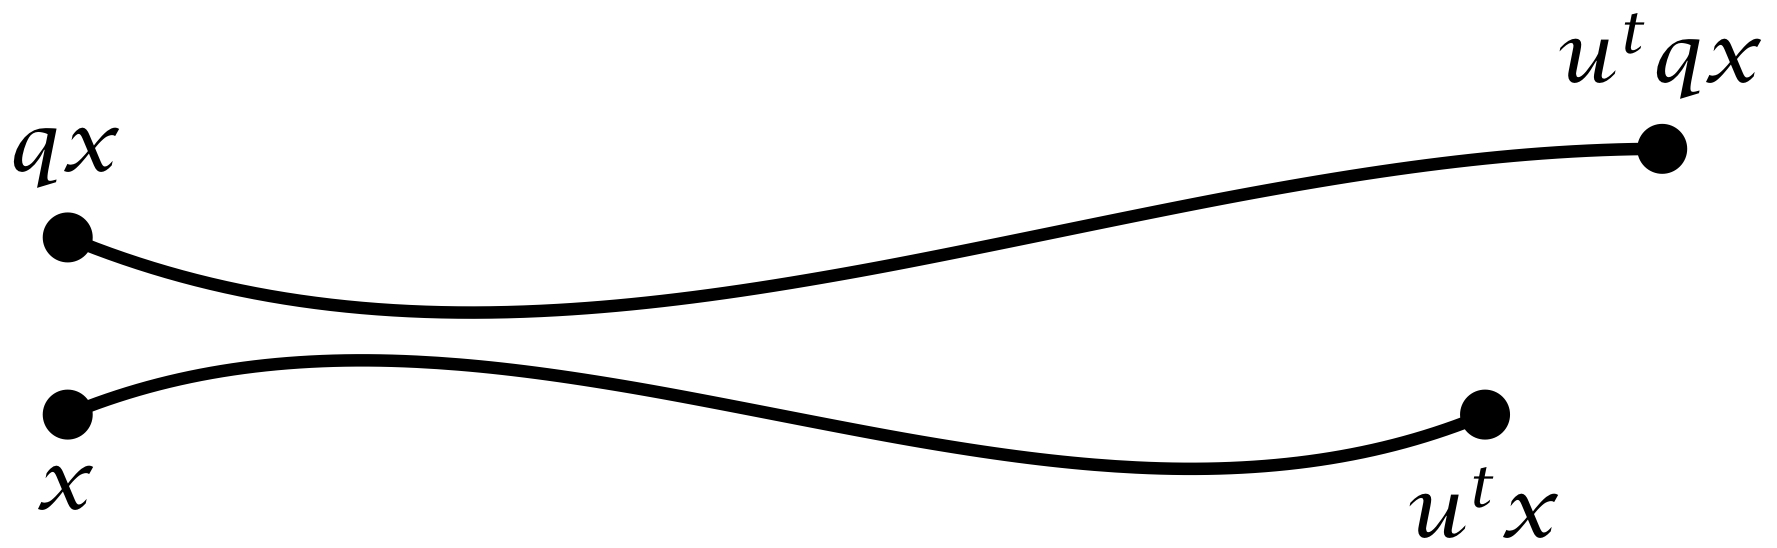
\includegraphics{PDF/movapart.jpg}
 \caption{The $u^t$-orbits of two nearby orbits.}
 \label{movapart}
 \end{center}
 \end{figure}
%texpreamble
%("  \usepackage{amsmath}
% \usepackage[LY1]{fontenc}
% \usepackage[expert,LY1,mylucidascale]{mylucidabr}
% ");
%defaultpen(  fontcommand("\normalfont") + fontsize(10) ); 
%
%from graph access *;
%unitsize(1.5cm);
%
%real linethick = 1.5;
%real dotthick = 12;
%dotfactor=12;
%
%pair x = (0,0), qx = (0,0.5);
%dot( x ); dot( qx); label( "$x$", x, 2*S); label( "$qx$", qx, 2*N); 
%
%pair ux = (4,0), uqx = (4.5,0.75);
%dot( ux ); dot( uqx); label( "$u^tx$", ux, 2*S); label( "$u^tqx$", uqx, 2*N); 
%
%draw( x{ENE}..{ENE}ux , linewidth(linethick) );
%draw( qx{ESE}..{E}uqx , linewidth(linethick) );
 \begin{itemize}
 \item To get from~$x$ to~$qx$, one multiplies by~$q$; therefore 
 	$$d(x,qx) = \|q - \Id \| .$$
 \item To get from $u^t x$ to~$u^t q x$, one multiplies by $u^t q u^{-t}$;
therefore 
 $$d( u^t x, u^t q x) = \|u^t q u^{-t} - \Id \| .$$
 (Actually, this equation only holds when the right-hand side is small --- there are infinitely many elements~$g$ of~$G$ with $g u^t x = u^t q x$, and the distance is obtained by choosing
the smallest one, which may not be $u^t q u^{-t}$ if $t$ is large.)
 \end{itemize}
 Letting
 $$ q - \Id = \begin{bmatrix}\mathsf{a} &\mathsf{b} \\ \mathsf{c} & \mathsf{d} \end{bmatrix}
,$$
 a simple matrix calculation shows that
 \begin{align} \label{ConjByU}
 u^t q u^{-t} - \Id = \begin{bmatrix}
 \mathsf{a} -\mathsf{b} t & \mathsf{b} \\
 \mathsf{c}  + (\mathsf{a} -\mathsf{d})t - \mathsf{b} t^2 & \mathsf{d} + \mathsf{b} t
 \end{bmatrix}
 .
  \end{align}

\begin{notation}
 For convenience, let $x_t = u^t x$ and $y_t = u^t y$.
 \end{notation}

Consider the right-hand side of \cref{ConjByU}, with $\mathsf{a}$, $\mathsf{b}$,
$\mathsf{c}$, and~$\mathsf{d}$ very small. Indeed, let us say they are
\index{infinitesimal}infinitesimal (too small to see). As $t$~grows, it is
the quadratic term in the bottom left corner that will be the first matrix entry to attain
macroscopic size. Comparing with the definition
of~$u^t$ \csee{ShearingNotation}, we see that this is exactly the direction
of the $u^t$-orbit. Therefore:


\begin{prop}[{(\index{shearing property}{Shearing Property})}]
\label{ShearingSL2R}
 The fastest \term{relative motion} between two
\term[nearby points|)]{nearby points} is parallel to the orbits of the flow.
 \end{prop}

 \begin{figure}[ht]
 \begin{center}
 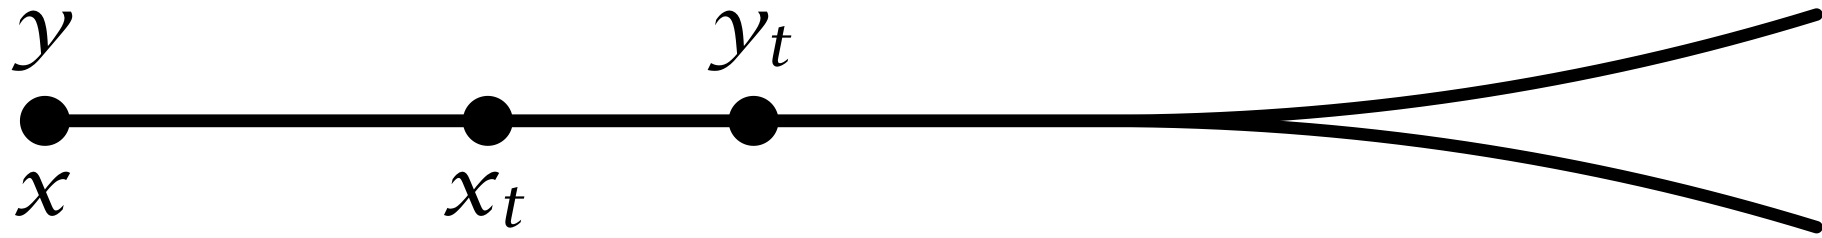
\includegraphics{PDF/shearing.jpg}
 \caption{Shearing: If two points start out so close together that we
cannot tell them apart, then the first difference we see will be that one
gets ahead of the other, but (apparently) following the same path. It is
only much later that we will be able to detect any difference between their paths.}
 \label{shearing}
 \end{center}
 \end{figure}
%texpreamble
%("  \usepackage{amsmath}
% \usepackage[LY1]{fontenc}
% \usepackage[expert,LY1,mylucidascale]{mylucidabr}
% ");
%defaultpen(  fontcommand("\normalfont") + fontsize(10) ); 
%
%from graph access *;
%unitsize(1.5cm);
%
%real linethick = 1.5;
%real dotthick = 12;
%dotfactor=12;
%
%real b = 0.3;
%pair x = (0,0), xt = (1.25,0), yt = (2,0);
%pair split = (3,0), xend = (5,-b), yend = (5,b);
%
%dot( x ); dot( xt); dot(yt);
%
%draw( x{E}..{E}split{E}..yend , linewidth(linethick) );
%draw( x{E}..{E}split{E}..xend , linewidth(linethick) );
%
%label( "$x$", x, 2*S); label( "$y$", x, 2*N); 
%label( "$x_t$", xt, 2*S); label( "$y_t$", yt, 2*N); 

\begin{rems} \ 
\noprelistbreak
\begin{enumerate}
\item The only exception to \cref{ShearingSL2R} is that if $q$ is in the centralizer $\czer_G(u^t)$, then $u^t q u^{-t} = q$ for
all~$t$; in this case, the points $x_t$ and~$y_t$ simply move along
together at exactly the same speed, with no \term{relative motion}.
\item  In contrast to the above discussion of~$u^t$, 
 \begin{itemize}
 \item the matrix $a^t$ is diagonal, 
 but
 \item the \term[largest!term]{largest entry} in 
 	$$ a^t q a^{-t} = \begin{bmatrix}
 \mathsf{a} & e^{2t} \mathsf{b} \\
e^{-2t} \mathsf{c}  & \mathsf{d} 
 \end{bmatrix} $$
is an off-diagonal entry,
 \end{itemize}
 so, under the action of the diagonal group, points move apart (at
exponential speed) in a direction transverse to the orbits
\csee{expdivfig}. 
\end{enumerate}
 \end{rems}

 \begin{figure}[ht]
 \begin{center}
 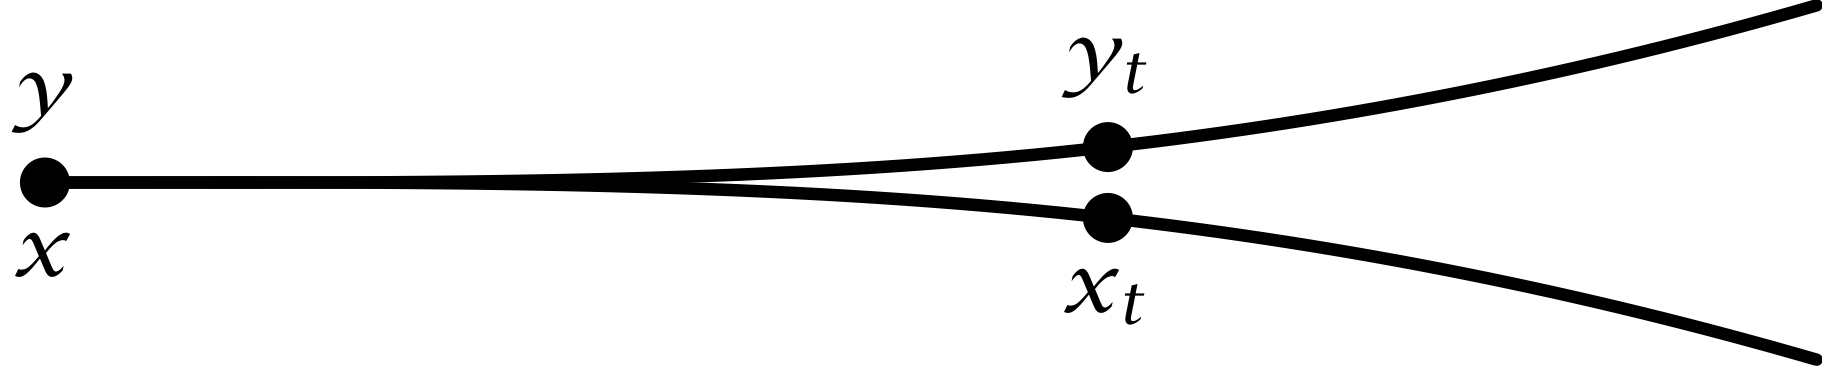
\includegraphics{PDF/expdiv.jpg}
 \caption{Divergence under a diagonal subgroup: when two points start out so close
together that we cannot tell them apart, the first difference we see
will be in a direction transverse to the orbits.}
 \label{expdivfig}
 \end{center}
 \end{figure}
%texpreamble
%("  \usepackage{amsmath}
% \usepackage[LY1]{fontenc}
% \usepackage[expert,LY1,mylucidascale]{mylucidabr}
% ");
%defaultpen(  fontcommand("\normalfont") + fontsize(10) ); 
%
%from graph access *;
%unitsize(1.5cm);
%
%real linethick = 1.5;
%real dotthick = 12;
%dotfactor=12;
%
%real a = 0.1, b = 0.5;
%pair x = (0,0), xt = (3,-a), yt = (3,a);
%pair xend = (5,-b), yend = (5,b);
%
%dot( x ); dot( xt); dot(yt);
%
%draw( x{E}..yt..yend , linewidth(linethick) );
%draw( x{E}..xt..xend , linewidth(linethick) );
%
%label( "$x$", x, 2*S); label( "$y$", x, 2*N); 
%label( "$x_t$", xt, 2*S); label( "$y_t$", yt, 2*N); 

The Shearing Property \pref{ShearingSL2R} shows that the direction of \term[relative
motion!fastest]{fastest relative motion} is along~$u^t$. However, in the
proof of Ratner's Theorems, it turns out that we wish to ignore
motion \emph{along} the orbits, and consider, instead, only the
\index{component, transverse}component of the relative motion that is
\defit[transverse divergence]{transverse} (or perpendicular) to the
orbits of~$u^t$. This direction, by definition, does not belong to
$\{u^t\}$. 

\begin{defn}
Suppose, as before, that $x$ and~$y$ are two points in
$X$ with $x \approx y$. Then, by continuity, $x_t \approx
y_t$ for a long time. Eventually, we will be able to see a difference
between $x_t$ and~$y_t$. The \term[shearing property!in
$\SL(2,\real)$]{Shearing Property} \pref{ShearingSL2R} tells us that, when
this first happens, $y_t$ will be indistinguishable from some point on the
orbit of~$x$; that is, $y_t \approx x_{t'}$ for some~$t'$. This will
continue for another long time (with $t'$ some function of~$t$), but we can
expect that $y_t$ will eventually diverge from the orbit of~$x$ --- this
is \defit[transverse divergence]{transverse divergence}. (Note that this
transverse divergence is a \term[second-order effect]{second-order
effect}; it is only apparent after we mod out the relative motion along
the orbit.) Letting $x_{t'}$ be the point on the orbit of~$x$ that is
closest to~$y_t$, we write $y_t = g x_{t'}$ for some $g \in G$. Then $g -
\Id$ represents the transverse divergence. When this transverse divergence
first becomes macroscopic, we wish to understand which of the matrix
entries of $g - \Id$ are macroscopic.
 \end{defn}

 In the matrix on the right-hand side of \cref{ConjByU}, we have already observed
that the \term[largest!entry]{largest entry} is in the bottom left corner,
the direction of~$\{u^t\}$. If we ignore that entry, then the two diagonal
entries are the largest of the remaining entries. The diagonal corresponds to the
subgroup~$\{a^t\}$. Therefore, the fastest
\defit[transverse divergence]{transverse} divergence is in the
direction of $\{a^t\}$. Notice that $\{a^t\}$
\term[normalizer]{normalizes}~$\{u^t\}$.


\begin{prop} \label{High1DTransN}
 The fastest \defit[transverse divergence]{transverse} motion is
along some direction in the \term{normalizer} of~$u^t$.

More precisely, if $x,y \in X$, with $x \approx y$, and $r > 0$ is much smaller than the injectivity radius of~$X$, then either:
	\begin{enumerate}
	\item there exist large $t,t' \in \real$ and $g \in \nzer_G\bigl( \{u^t\} \bigr)$ such that
	$$ \text{$u^t y \approx g u^{t'} x$ and\/ $\| g \| = d \bigl(g, \{u^t\} \bigr) = r$,} $$
	or
	\item for all $t \in \real$, there exists $t' \in \real$, such that $u^t y \approx u^{t'} x$ \textup(i.e., there is no transverse motion, only shearing\textup).
	\end{enumerate}
 \end{prop}

To illustrate how understanding the transverse motion can be useful, let us prove a very special case of Ratner's Orbit-Closure Theorem \pref{Ratner-OrbitClosure}.

\begin{prop} \label{MinSetIsUOrbit}
Let $C = \closure{\{u^t\}x}$, for some $x \in X$, and assume
	\begin{itemize}
	\item $C$ is a \defit[minimal!closed, invariant set]{minimal} $u^t$-invariant closed subset of~$X$ 
	\textup(this means that no nonempty, proper, closed subset of~$C$ is\/ $\{u^t\}$-invariant\/\textup),
	and
	\item $\{\, g \in G \mid gC = C \,\} =  \{u^t\}$.
	\end{itemize}
Then $C = \{u^t\}x$, so $C$~is a submanifold of~$X$.
\end{prop}

\begin{proof}
We wish to show $C \subseteq \{u^t\}x$, but \cref{MinSetIsUOrbit-CcapCg=0Ex} implies that it suffices to prove only the weaker statement that $C \subseteq \nzer_G\bigl( \{u^t\} \bigr) \, x$.

Suppose $C \not\subseteq \nzer_G\bigl( \{u^t\} \bigr) \, x$. Then, since $C$ is connected, there exists $y \in C$, with $y \approx x$, but $y \notin \nzer_G\bigl( \{u^t\} \bigr) \, x$.
From \cref{High1DTransN}, we see that there exist $t,t' \in \real$ and 
	$$ \text{$g \in \nzer_G\bigl( \{u^t\} \bigr)$, with $g \notin \{u^t\}$, such that
	$ u^t y \approx g u^{t'} x $.} $$
For simplicity, let us pretend that 
	$$\text{$u^t y$ is \emph{equal} to $g u^{t'} x$} , $$
rather than merely being approximately equal \csee{MinSetIsUOrbit-xu=yuEx}. Then we have $C \cap gC \neq \emptyset$ (because $u^t y \in C$ and $g u^{t'} x \in g C$).
This contradicts \cref{MinSetIsUOrbit-CcapCg=0Ex}.
\end{proof}

\begin{exercises}

\item \label{MinSetIsUOrbit-CcapCg=0Ex}
Under the assumptions of \cref{MinSetIsUOrbit}, show: 
	$$ \text{if $g \in \nzer_G\bigl( \{u^t\} \bigr)$, but $g \notin \{u^t\}$, then $C \cap gC = \emptyset$.} $$ (In particular, $g x \notin C$.)
\hint{$gC$ is $u^t$-invariant (because $g \in \nzer_G\bigl( \{u^t\} \bigr)$), so $C \cap gC$ is a $u^t$-invariant subset of the minimal set~$C$.}

\item \label{MinSetIsUOrbit-xu=yuEx}
Complete the proof of \cref{MinSetIsUOrbit} by eliminating the pretense that $u^t y$ is \emph{equal} to $g u^{t'} x$.
\hint{The compact sets $C$ and $\{\, g \in \nzer_G\bigl( \{u^t\} \bigr) \mid \|g\| = d \bigl( g,\{u^t\} \bigr) = r \,\} \cdot C$ are disjoint, so it is impossible for a point in one set to be arbitrarily close to a point in the other set.}

\end{exercises}




\begin{notes}

\Cref{Ratner-OrbitClosure} is due to M.\,Ratner \cite{Ratner-OrbitClosure}, under the assumption that $V$ is either unipotent or connected. 
(A shorter proof can be found in \cite{MargulisTomanov-InvtMeas}.)
This additional hypothesis was removed by N.\,Shah \cite{Shah-GenByUnip} (except for a technical problem involving Conclusions \pref{Ratner-OrbitClosure-AlmConn} and~\pref{Ratner-OrbitClosure-probmeas} that was resolved in \cite[Cor.~3.5.4]{KleinbockShahStarkov}).

See \cite{Morris-RatnersThms} for a more thorough introduction to Ratner's Theorems, their proofs, and some applications.

See \cite[Lem.~2]{Starkov-StructOrbAndRagConj} for the construction of orbits whose closure is not a submanifold, demonstrating the pathology in \cref{MustBeUnip,FractalInHyper3Mfld}.
	%(originally Morse?)
However, it was conjectured by G.\,A.\,Margulis \cite[\S1.1]{Margulis-problems} that certain analogues of Ratner's Theorems are valid in some situations where the subgroup~$V$ is a split torus of dimension~$> 1$; see \cite[\S4.4c]{KleinbockShahStarkov} and~\cite{Maucourant-Nonhomog} for references on this open problem and its applications.

\Cref{GoodClosure(hyper)} was proved by N.\,Shah \cite{Shah-TotallyGeodesic}. The generalization in \fullcref{GoodClosure(LocSymm)}{closure} is due to T.\,Payne \cite{Payne-Closures}.

\Cref{OppenheimConj} is due to G.\,A.\,Margulis \cite{Margulis-Oppenheim}.
See \cite{Margulis-OppenheimSurvey} for a survey of its history and later related developments.

\Cref{ProdLattsDense} was discovered by N.\,Shah \cite[Cor.~1.5]{Shah-GenByUnip}. This consequence of Ratner's Theorem played an important role in \cite{Vatsal-Heegner}.

\Cref{Ratner-Equidistribution} is due to M.\,Ratner \cite{Ratner-OrbitClosure}.

\Cref{Ratner-MeasClass} was proved by M.\,Ratner \cite{Ratner-MeasClass} in the case where $V$ is either unipotent or connected. 
(See \cite{Einsiedler-RatnerSL2R} for a shorter and more self-contained proof in the case where $V \iso \SL(2,\real)$.)
The general case is due to N.\,Shah \cite{Shah-GenByUnip}.

\Cref{UnipotentIsomorphismRigidity} was proved by M.\,Ratner \cite{Ratner-UnipRigidity} if $G_1 \iso G_2 \iso \SL(2,\real)$. The general case is due to D.\,Witte \cite{Witte-UnipRigidity}.

\Cref{UniqErg->UnifDist} is a special case of a classical result in Ergodic Theory that can be found in textbooks such as \cite[Thm.~6.19]{Walters}.

See \cite{BenoistQuint-StatMeas3} for the work of Y.\,Benoist and J.--F.\,Quint mentioned in \fullcref{MeasClassRems}{BenoistQuint}. Shah's suggestion about Zariski closures appears in \cite[end of \S1, p.~232]{Shah-GenByUnip}.

The discussion of shearing in \cref{RatnerShearingSect} is excerpted from \cite[\S1.5]{Morris-RatnersThms}, except that \cref{MinSetIsUOrbit} is a variant of \cite[Prop.~1.6.10]{Morris-RatnersThms}.

\end{notes}


\begin{references}{99}

\bibitem{BenoistQuint-StatMeas3}
Y.\,Benoist and J.--F.\,Quint:
Stationary measures and invariant subsets of homogeneous spaces~(III),
\emph{Ann. of Math.} (2) 178 (2013), no.~3, 1017--1059.
\MR{3092475},
\maynewline
\url{http://dx.doi.org/10.4007/annals.2013.178.3.5 }

\bibitem{Einsiedler-RatnerSL2R}
M.\,Einsiedler:
Ratner's theorem on ${\mathrm{SL}}(2,\mathbb{R})$-invariant measures,
\emph{Jahresber. Deutsch. Math.-Verein.} 108 (2006), no.~3, 143--164. 
\MR{2265534} % no URL available @@@

\bibitem{KleinbockShahStarkov}
D.\,Kleinbock, N.\,Shah, and A.\,Starkov:
Dynamics of subgroup actions on homogeneous spaces of Lie groups and applications to number theory,
in B.\,Hasselblatt and A.\,Katok, eds.:
\emph{Handbook of Dynamical Systems, Vol. 1A.}
North-Holland, Amsterdam, 2002, pages~813--930.
\MR{1928528}

\bibitem{Margulis-Oppenheim}
G.\,A.\,Margulis:
Formes quadratriques ind\'efinies et flots unipotents sur les espaces homog\`enes,
\emph{C. R. Acad. Sci. Paris S\'er.~I Math.} 304 (1987), no.~10, 249--253. 
\MR{0882782} % no URL available @@@

\bibitem{Margulis-OppenheimSurvey}
G.\,A.\,Margulis:
Oppenheim Conjecture,
in  M.\,Atiyah and D.\,Iagolnitzer, eds.:
\emph{Fields Medallists' Lectures.}
World Sci. Publ., River Edge, NJ, 1997, pp.~272--327.
\MR{1622909}

\bibitem{Margulis-problems}
G.\,A.\,Margulis:
Problems and conjectures in rigidity theory,
in V.\,Arnold et al., eds.:
\emph{Mathematics: Frontiers and Perspectives.}
Amer. Math. Soc., Providence, RI, 2000, pp.~161--174.
\MR{1754775 }

\bibitem{MargulisTomanov-InvtMeas}
G.\,A.\,Margulis and G.\,M.\,Tomanov:
Invariant measures for actions of unipotent groups over local fields on homogeneous spaces,
\emph{Invent. Math.} 116 (1994) 347--392.
\MR{1253197},
\maynewline
\url{http://eudml.org/doc/144192}
%\url{http://www.digizeitschriften.de/dms/resolveppn/?PPN=GDZPPN002111802}

\bibitem{Maucourant-Nonhomog}
F.\,Maucourant:
A non-homogeneous orbit closure of a diagonal subgroup,
\emph{Ann. of Math.} (2) 171 (2010), no.~1, 557--570.
 \MR{2630049},
 \maynewline
 \url{http://dx.doi.org/10.4007/annals.2010.171.557}

\bibitem{Morris-RatnersThms}
D.\,W.\,Morris:
\emph{Ratner's Theorems on Unipotent Flows.}
%Chicago Lectures in Mathematics. 
University of Chicago Press, Chicago, IL, 2005.
ISBN 0-226-53984-9,
\MR{2158954},
\maynewline
\url{http://arxiv.org/abs/math/0310402}

\bibitem{Payne-Closures}
T.\,L.\,Payne:
Closures of totally geodesic immersions into locally symmetric spaces of noncompact type,
\emph{Proc. Amer. Math. Soc.}  127  (1999),  no.~3, 829--833.
\MR{1468202},
\maynewline
\url{http://dx.doi.org/10.1090/S0002-9939-99-04552-9}

\bibitem{Ratner-UnipRigidity}
M.\,Ratner:
Rigidity of horocycle flows,
\emph{Ann. of Math.} 115  (1982), no.~3, 597--614. 
\MR{0657240},
\maynewline
\url{http://www.jstor.org/stable/2007014}

\bibitem{Ratner-MeasClass}
M.\,Ratner:
On Raghunathan's measure conjecture,
\emph{Ann. of Math.} 134 (1991), no.~3, 545--607. 
\MR{1135878},
\maynewline
\url{http://www.jstor.org/stable/2944357}

\bibitem{Ratner-OrbitClosure}
M.\,Ratner:
Raghunathan's topological conjecture and distributions of unipotent flows,
\emph{Duke Math.~J.} 63 (1991), no.~1, 235--280. 
\MR{1106945},
\maynewline
\url{http://dx.doi.org/10.1215/S0012-7094-91-06311-8}

\bibitem{Shah-TotallyGeodesic}
N.\,Shah:
Closures of totally geodesic immersions in manifolds of constant negative curvature,
in \'E.\,Ghys, A.\,Haefliger and A.\,Verjovsky, eds.:
\emph{Group Theory from a Geometrical Viewpoint (Trieste, 1990),}
World Sci. Publ., River Edge, NJ, 1991, pp.~718--732.
\MR{1170382}

\bibitem{Shah-GenByUnip}
N.\,Shah:
Invariant measures and orbit closures on homogeneous spaces for actions of subgroups generated by unipotent elements,
in S.\,G.\,Dani, ed.:
\emph{Lie Groups and Ergodic Theory (Mumbai, 1996),}
%Tata Inst. Fund. Res. Stud. Math., 14, 
Tata Inst. Fund. Res., Bombay, 1998,
pp.~229--271.
\MR{1699367}

\bibitem{Starkov-StructOrbAndRagConj}
A.\,N.\,Starkov:
Structure of orbits of homogeneous flows and the Ragunatana conjecture,
\emph{Russian Math. Surveys} 45 (1990), no.~2, 227--228. 
 (Translated from \emph{Uspekhi Mat. Nauk} 45 (1990), no.~2(272), 219--220.)
\MR{1069361},
\maynewline
\url{http://dx.doi.org/10.1070/RM1990v045n02ABEH002338}

\bibitem{Vatsal-Heegner}
V.\,Vatsal:
Uniform distribution of Heegner points,
\emph{Invent. Math.} 148 (2002)  1--46.
\MR{1892842},
\maynewline
\url{http://dx.doi.org/10.1007/s002220100183}

\bibitem{Walters}
 P.\,Walters:
 \emphit{An Introduction to Ergodic Theory.}
% Graduate Texts in Mathematics, 79. 
 Springer, New York, 1982
 ISBN 0-387-90599-5,
 \MR{0648108}

\bibitem{Witte-UnipRigidity}
D.\,Witte:
Rigidity of some translations on homogeneous spaces,
\emph{Invent. Math.}  81  (1985),  no.~1, 1--27.
\MR{0796188},
\maynewline
\url{http://eudml.org/doc/143244}
%\url{http://www.digizeitschriften.de/dms/resolveppn/?PPN=GDZPPN002101769}


\end{references}
